\documentclass{standalone}
\usepackage{tikz}

\begin{document}
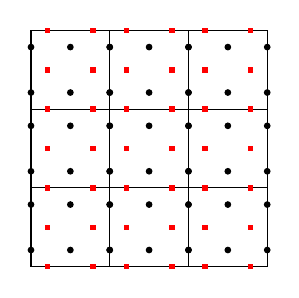
\begin{tikzpicture}[square/.style={rectangle, inner sep=1pt, fill=red}]
	\draw (0,0) grid (3,3); 
	\foreach \i in {0,1,2} {
		\foreach \j in {0,1,2} {
			\foreach \x in {0,.5,1} {
				\foreach \y in {0.21132487, 0.78867513} {
					\filldraw[black] (\x+\i, \y+\j) circle[radius=1pt]; 
					\node[square] at (\y+\i, \x+\j) {}; 
				}
			} 
		}
	}
\end{tikzpicture}
\end{document}